
\fancyhead[C]{Section 15.1}
\fancyhead[R]{\dayfifteen}

\section*{\centering Chapter 15.1: Double Integrals on Rectangles}
\textbf{I1: Double \& Triple Integrals.} I can set up double and triple integrals as iterated integrals over any region. I can sketch regions based on a given iterated integral.\\\\
\textbf{I2: Iterated Integrals.} I can compute iterated integrals of two and three variable functions, including applying Fubini's Theorem to change the order of integration of an iterated integral.

\subsection*{Mechanics}
\begin{enumerate}
    \item \question{Compute $\displaystyle \iint_R (xy-3xy^2) \ dA$, where  $R$ is the square $0 \leq x \leq 2,1 \leq y \leq 2$.}{-11
    }
    {% solution goes here
    } 
    \item \question{Use Fubini's Theorem to evaluate the integral
	\begin{equation*}
	    \int_0^1 \int_0^3 xe^{xy}\ dx\ dy 
	\end{equation*} 
    Why was it a good idea to exchange the order of integration?}{% answer goes here
    }
    {% solution goes here
    } 
    \item \question{Find the volume of the region bounded above by the paraboloid $z = 16 - x^2 - y^2$ and below by the square 
$R: 0 \leq x \leq 2, 0 \leq y \leq 2$.}{% answer goes here
    }
    {% solution goes here
    } 
\end{enumerate}
\subsection*{Extensions}
\begin{enumerate}[resume]
\item \question{Evaluate the double integral $\iint_R (4-2y)\ dA$, where $R=[0,1]\times[0,1]$ \textbf{without integrating} by identifying it as the volume of a solid \textit{[Hint: It is a prism cut by some plane.]}}{% answer goes here
    }
    {% solution goes here
    } 

\item \question{The integral $\iint_R \sqrt{9-y^2}$, where $R=[0,4]\times[0,2]$, represents the volume of a solid.  Sketch the solid.}{% answer goes here
    }
    {% solution goes here
    } 
	
	\item \question{This problem explores a failure of Fubini's theorem. Consider the two iterated integrals, which differ by swapping the order of integration:
	\begin{equation*}
	\int_0^1 \int_0^1 \frac{x^2-y^2}{(x^2+y^2)^2}\ dy\ dx \quad \textrm{ and }\quad \int_0^1 \int_0^1 \frac{x^2-y^2}{(x^2+y^2)^2}\ dx\ dy \end{equation*}
    Use the fact that 
    \begin{equation*}
        \frac{\partial}{\partial y} \left(\frac{y}{x^2+y^2}\right)=\frac{\partial}{\partial x} \left(\frac{-x}{x^2+y^2}\right)= \frac{x^2-y^2}{(x^2+y^2)^2}
    \end{equation*}
    and that $\frac{d}{dt}\arctan(t) = 1/(1+t^2)$ to show that the iterated integrals are different. Why does Fubini's theorem fail? }
    {% answer goes here
    }
    {% solution goes here
    } 
	
\end{enumerate}
{}

\iftoggle{answers}{
\begin{center}{\large \textbf{Math 2551 Worksheet Answers: Double Integrals on Rectangles}}
\end{center}

\begin{enumerate}
	\item 
	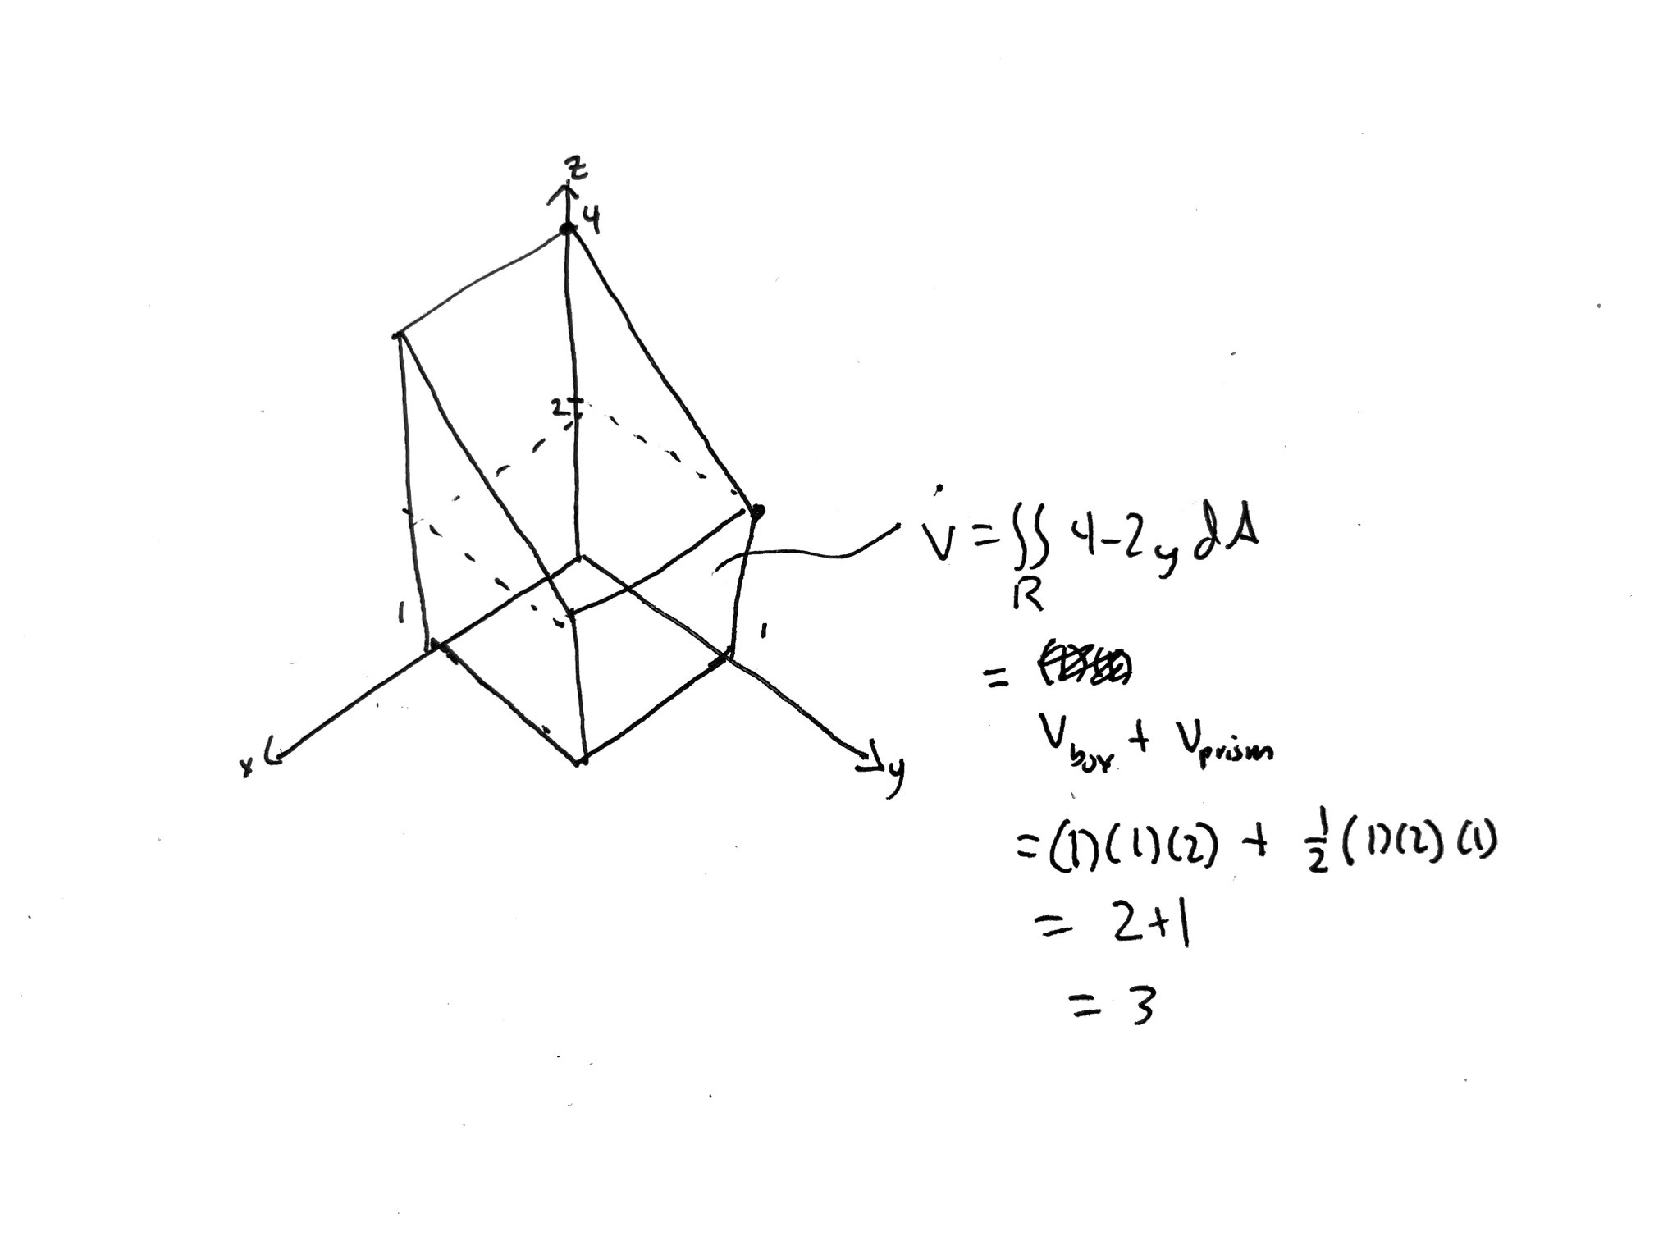
\includegraphics[scale=0.3]{ws_15_1_src.pdf}
	
	\item 
	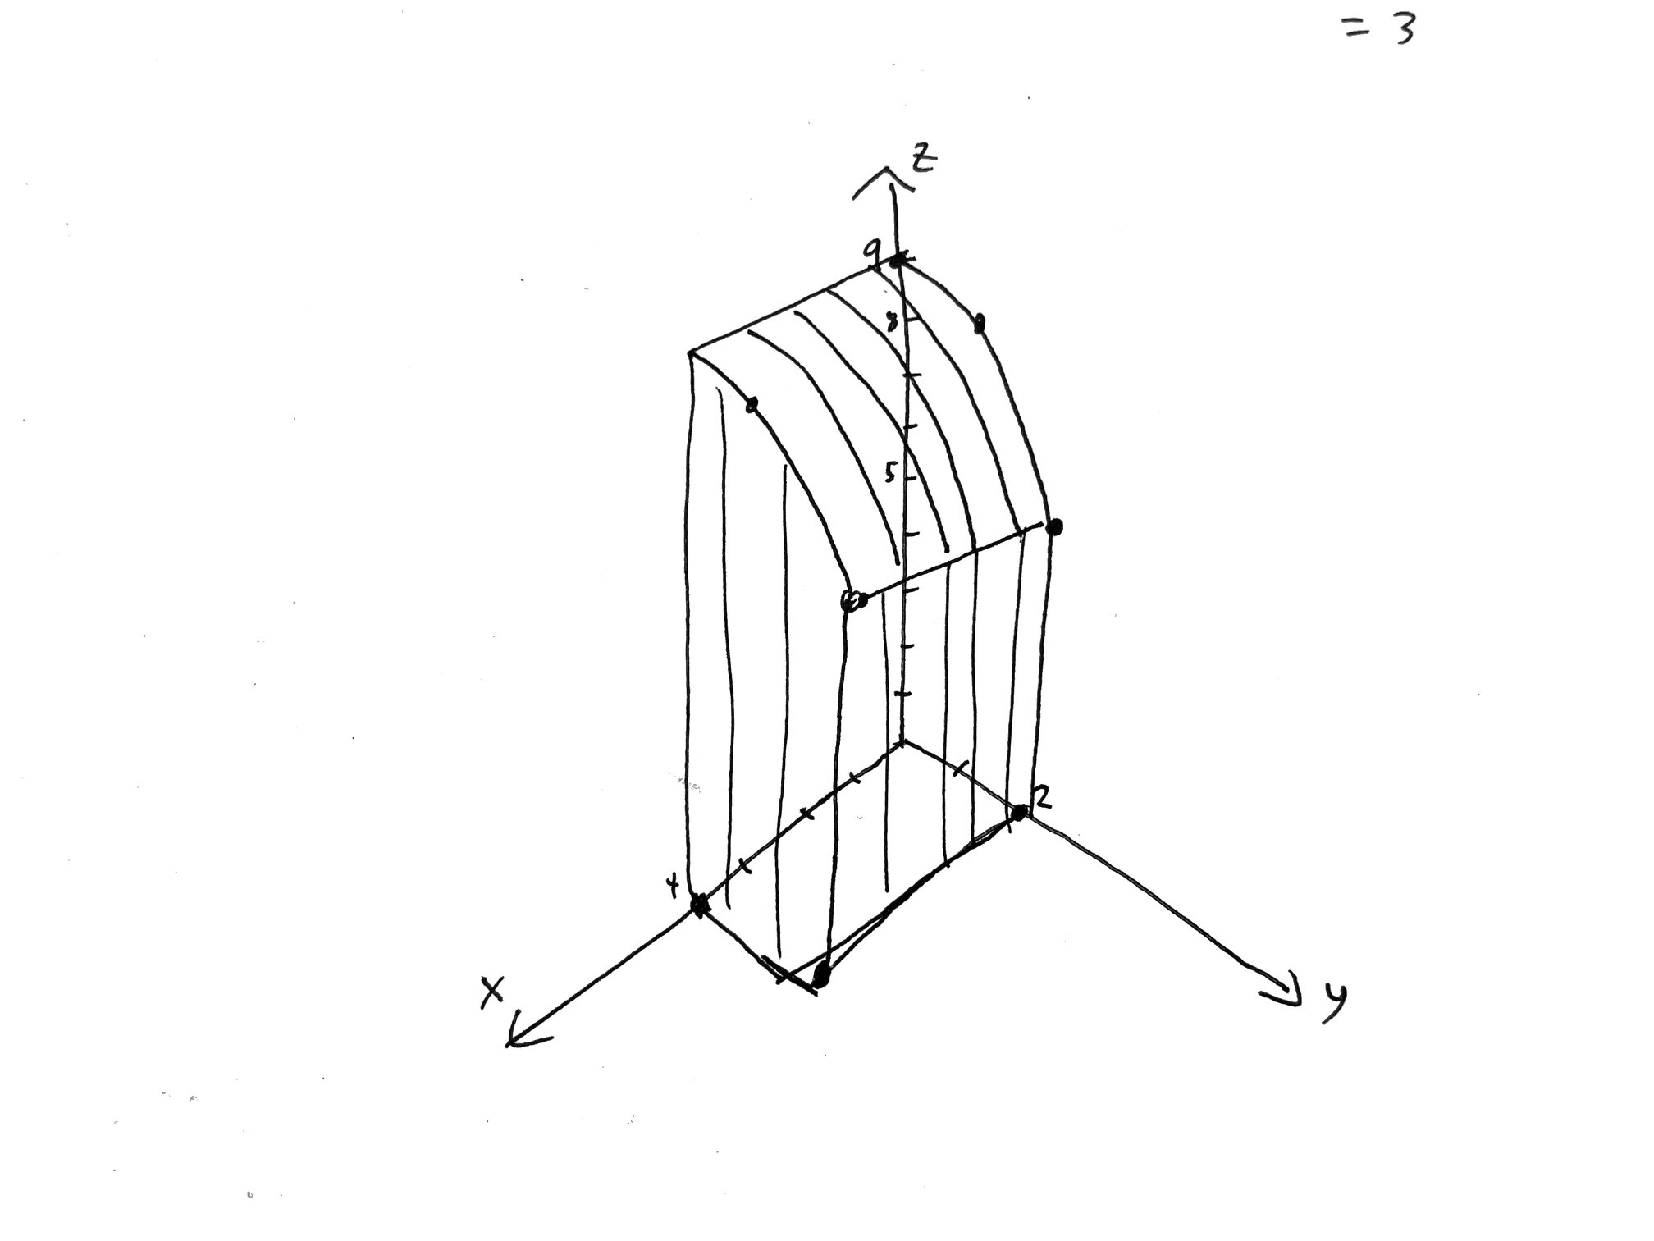
\includegraphics[scale=0.25]{ws_15_2_src.pdf}
	
	\item $9\ln(2)$
	
	\item $160/3$ cubic units.
	
		\item $e^3-4$

	\item The integrals evaluate to $\pi/4$ and $-\pi/4$ respectively.  This does not violate Fubini's theorem because this function is not continuous on $[0,1]\times[0,1]$ (it has an asymptote at $(0,0)$)
\end{enumerate}
}{}
\iftoggle{solutions}
{
Solutions go here in the same format.
}{}
